% Main result figures generated by experiments/make_paper_figures_v2.py from
% results/paper/paper_scale_v2. The PDF files are committed and render-checked
% by .github/workflows/aqng-paper-figures-v2.yml.

\begin{figure*}[t]
\centering
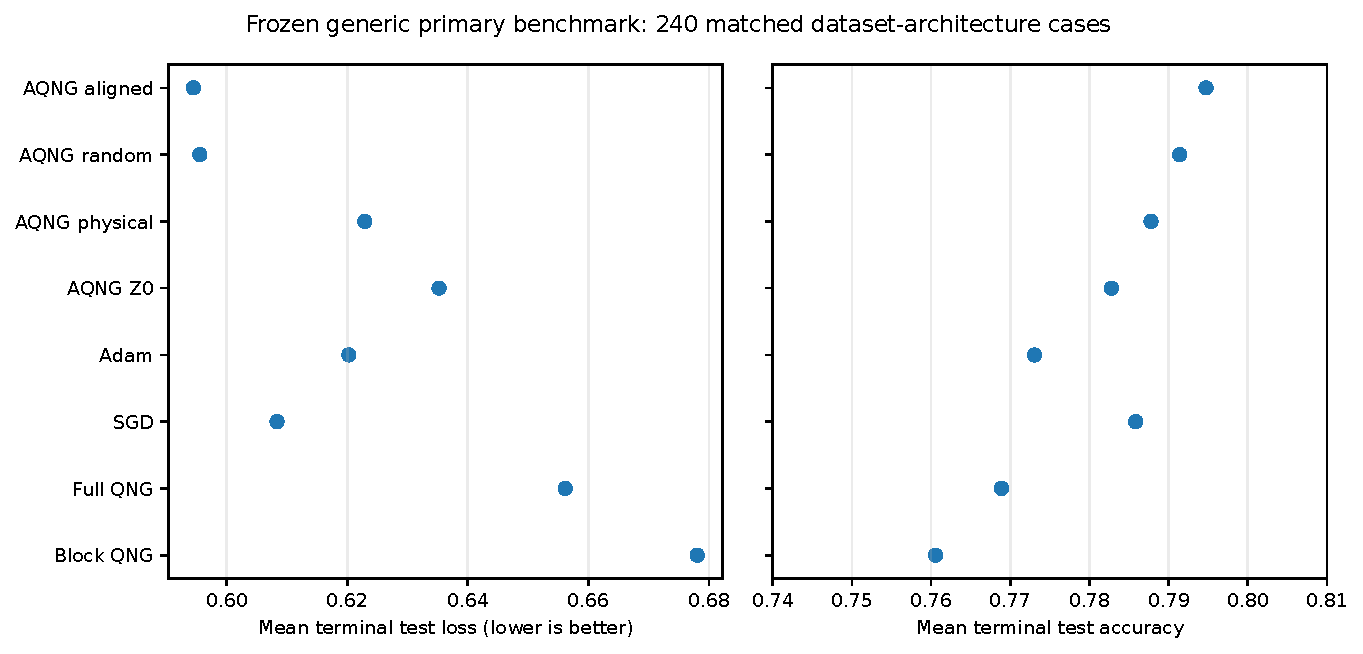
\includegraphics[width=0.96\textwidth]{figures/generated/fig02_generic_primary.pdf}
\caption{Frozen generic primary benchmark pooled over the 240 nonconserving dataset--architecture cases. The primary protocol compares eight methods at matched data partitions and stochastic seeds. Aligned AQNG has the lowest pooled mean terminal test loss (0.5945) and highest pooled mean accuracy (0.7947), but random AQNG and SGD remain close. The pooled means are descriptive summaries; inferential claims use paired tests rather than treating all terminal rows as independent replicates.}
\label{fig:generic_primary}
\end{figure*}

\begin{figure*}[t]
\centering
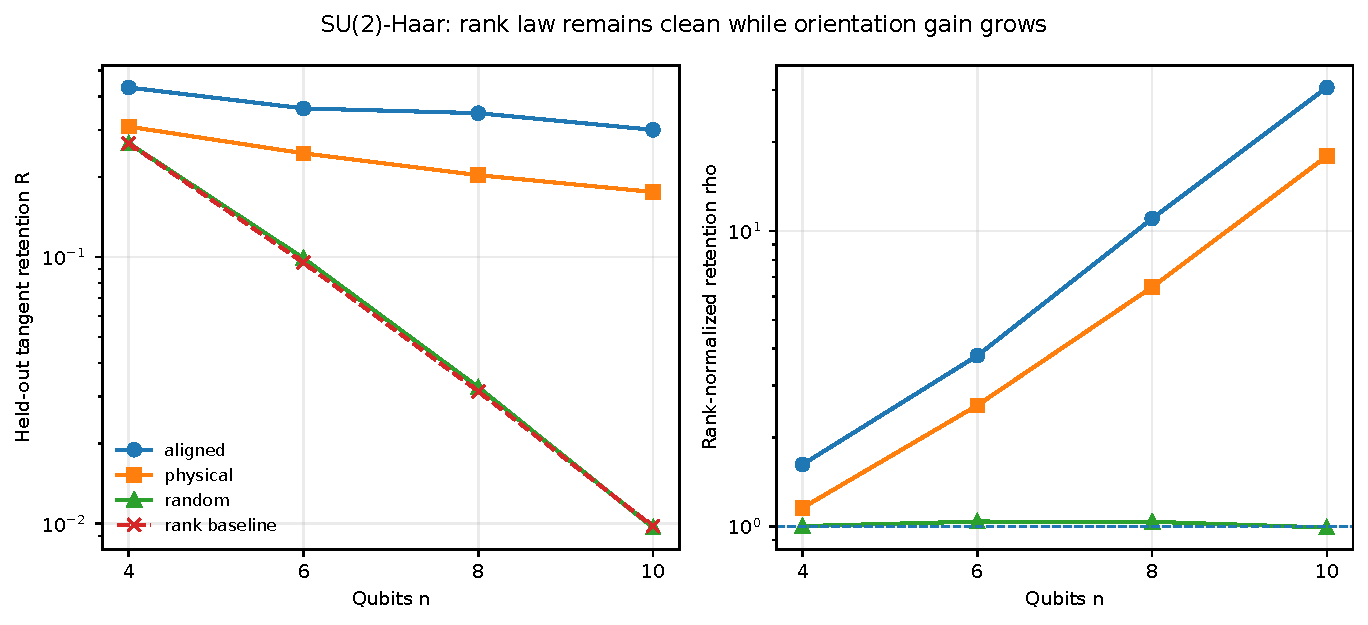
\includegraphics[width=0.96\textwidth]{figures/generated/fig03_scaling_geometry.pdf}
\caption{Qubit scaling of SU(2)-Haar readout geometry at fixed readout order. Left: held-out tangent retention $R$ for cross-fitted aligned, physical, and Haar-random equal-rank readouts, together with the rank-only baseline $r/N$. The baseline falls from $0.267$ at $n=4$ to $9.78\times10^{-3}$ at $n=10$, while the aligned readout still retains about $0.300$ at $n=10$. Right: rank-normalized retention $\rho$. The random control remains near $\rho=1$, whereas the physical and aligned readouts rise to approximately $17.9$ and $30.7$ at $n=10$. The growth is a task-conditioned orientation effect, not a claim that generic physical readouts violate the rank law.}
\label{fig:scaling_geometry}
\end{figure*}

\begin{figure*}[t]
\centering
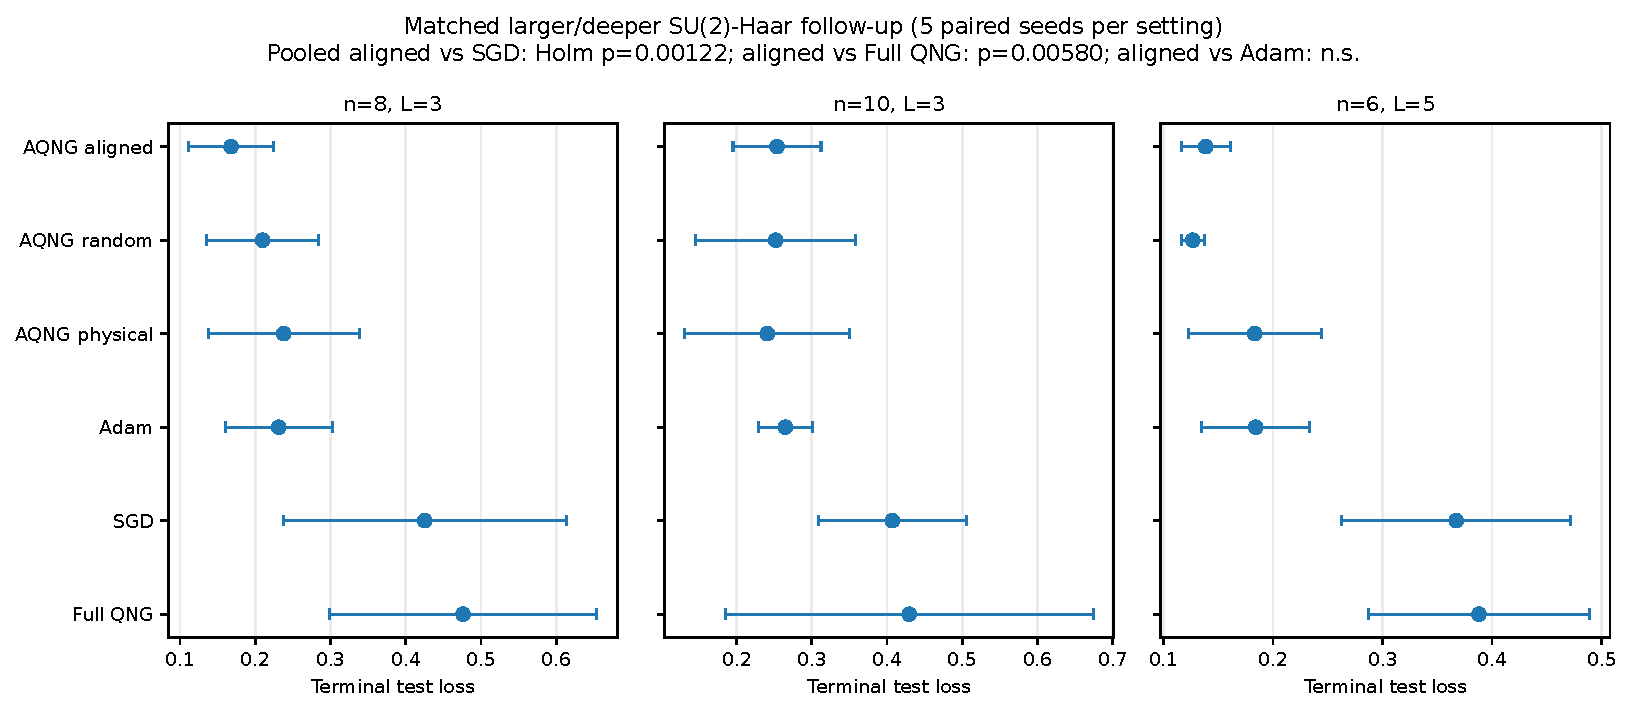
\includegraphics[width=0.98\textwidth]{figures/generated/fig04_large_deep.pdf}
\caption{Matched larger/deeper SU(2)-Haar follow-up. Error bars show the standard deviation across five paired seeds within each setting. Pooled over the 15 matched cells, aligned AQNG beats SGD in 15/15 cases with Holm-adjusted $p=1.22\times10^{-3}$ and full QNG in 14/15 with $p=5.80\times10^{-3}$. The aligned--Adam difference is smaller (10/15 wins) and is not statistically resolved. The follow-up therefore supports a robust advantage over SGD and the tested full-QNG baseline in these regimes, but not universal superiority over Adam.}
\label{fig:large_deep}
\end{figure*}

\begin{figure*}[t]
\centering
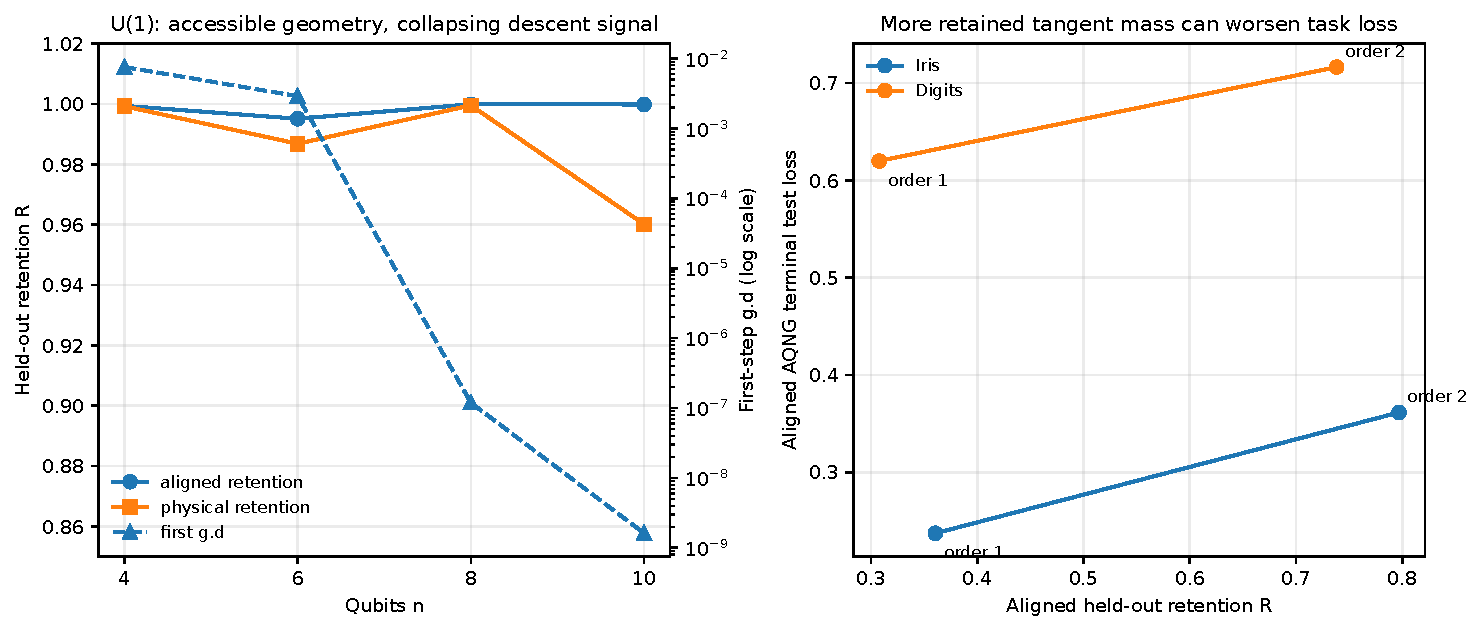
\includegraphics[width=0.98\textwidth]{figures/generated/fig05_accessibility_not_trainability.pdf}
\caption{Accessibility is not trainability. Left: in the half-filled $U(1)$ family, physical and cross-fitted aligned readouts retain nearly all held-out tangent mass over the tested scaling range, while the first-step $g^{\mathsf T}d$ diagnostic collapses by many orders of magnitude and terminal accuracy remains chance-like. Right: for SU(2)-Haar, increasing the readout from order one to order two moves both Iris and Digits toward substantially larger aligned retention but also larger terminal aligned-AQNG loss. Retention is therefore a geometric accessibility diagnostic, not a monotone task-performance objective.}
\label{fig:accessibility_not_trainability}
\end{figure*}

\begin{figure}[t]
\centering
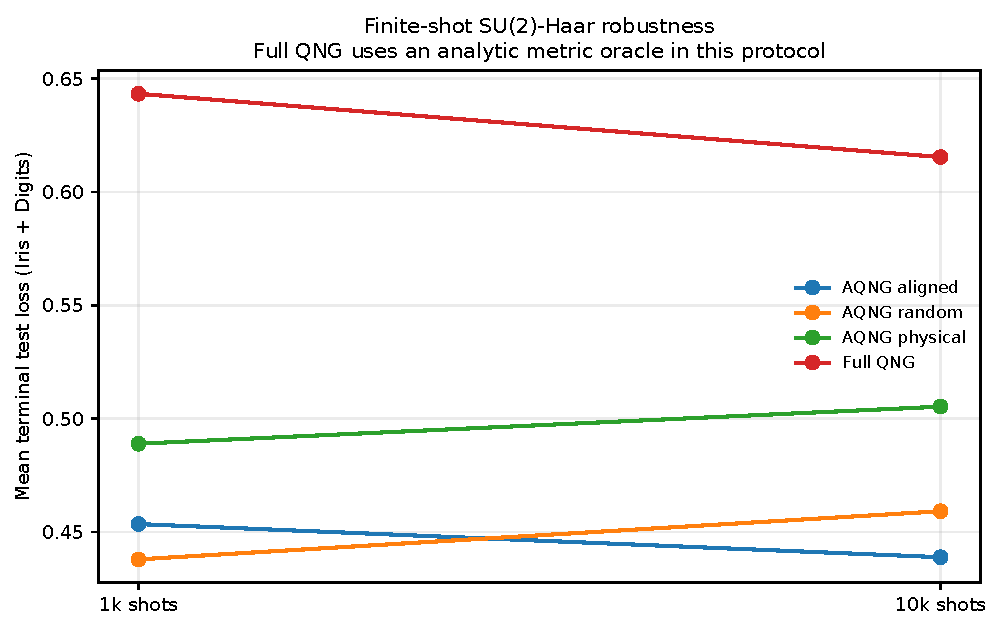
\includegraphics[width=0.98\columnwidth]{figures/generated/fig06_finite_shot.pdf}
\caption{Finite-shot SU(2)-Haar comparison averaged over the Iris and Digits finite-shot cells. AQNG remains competitive at both $10^3$ and $10^4$ shots in the tested protocol, without a monotone terminal-loss improvement as the shot count increases. Full QNG is included as an optimization reference but uses an analytic metric oracle in these finite-shot runs; the figure must therefore not be interpreted as a hardware-fair resource comparison.}
\label{fig:finite_shot}
\end{figure}
